\section{Preprocessing}
\todo{Why did we do this?}

\subsection{E-Mail Parsing}
\todo{This is our simple technique}
\todo{
    \begin{itemize}
        \item Strip metadata
        \item Strip HTML
        \item Multipart Splitting
    \end{itemize}
}
\todo{Improvement?}

\subsection{Stemming}
Most words in the English language are derived from a {\it morphological root} that contains no prefixes or suffixes and conveys a very similar meaning to its derivation. A simple example of this is {\it subscriber} and {\it subscription} with their morphological root {\it subscribe}. 

If we can reduce all incoming words into their root form, we would be able to substantially reduce the number of dimensions for our model while also ensuring that words representing the same underlying feature are stored under the same value.

Unfortunately, such a task is quite hard and would probably require the creation of a very large lookup table for each word in the English language along with its root. This is due to the fact that the English language is not a formal language and does not follow a strict set of rules. 

We could however, take an approximation of the described process and instead derive the {\it stem} of each word. Like the morphological root, the stem is a representation of a words underlying meaning. However the stem does not guarantee to be a correct English word or generate the right root as its aim is simply to map variations of the same word to the same to item. 

For our Spam Filter implementation, we made use of the Porter Stemmer algorithm \cite{porter1980}, which in the authors on words is ``a process for removing the commoner morphological and inflexional endings from words in English process''. In simpler terms, it is capable of removing known suffixes from the end of words passed to it. The Porter Stemmer algorithm is available as open source code under the BSD License and is available under multiple languages, including Java.

Using the same examples used before, passing {\it subscriber} and {\it subscribe} to the Porter Stemmer would reduce both words to the stem {\it suscrib}. On the other hand, the word {\it subscription} will be wrongly mapped to a different stem {\it subscript}, which is an example of where the approximation fails to produce the correct result.

In terms of the Spam Filter implementation, using Porter Stemming on the given set of training emails reduced the number of words from 24813 wordsto 18932 stems (both after text pre-processing). This is a substantial reduction in the number of dimensions and plays a crucial role in ensuring that the classifier is able to train with the given documents in a short amount of time and without requiring large amounts of memory. It has also shown to improve classification performance. \todo{include some results - simple example I have is 0.973 with and 0.97 without.

\todo{Improvement?}

\subsection{Feature selection}
\todo{Is this really preprocessing?}

As the number of features generated by the input data is even very high after the previous preprocessing steps, we are going to minimise its number by trimming features which are (siginificantly) relevant for the classification quality.

\todo{\dots}

\begin{figure}[h!]
    \centering
    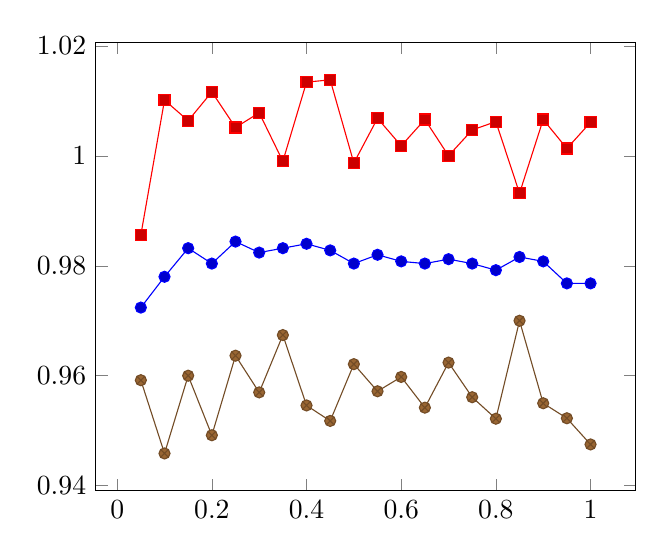
\begin{tikzpicture}
        \begin{axis}
             \addplot+[sharp plot] coordinates {
                (0.05, 0.972400)
                (0.10, 0.978000)
                (0.15, 0.983200)
                (0.20, 0.980400)
                (0.25, 0.984400)
                (0.30, 0.982400)
                (0.35, 0.983200)
                (0.40, 0.984000)
                (0.45, 0.982800)
                (0.50, 0.980400)
                (0.55, 0.982000)
                (0.60, 0.980800)
                (0.65, 0.980400)
                (0.70, 0.981200)
                (0.75, 0.980400)
                (0.80, 0.979200)
                (0.85, 0.981600)
                (0.90, 0.980800)
                (0.95, 0.976800)
                (1.00, 0.976800)
                };
             \addplot+[sharp plot] coordinates {
                (0.05, 0.972400+0.013206)
                (0.10, 0.978000+0.032125)
                (0.15, 0.983200+0.023186)
                (0.20, 0.980400+0.031215)
                (0.25, 0.984400+0.020746)
                (0.30, 0.982400+0.025424)
                (0.35, 0.983200+0.015799)
                (0.40, 0.984000+0.029394)
                (0.45, 0.982800+0.031010)
                (0.50, 0.980400+0.018287)
                (0.55, 0.982000+0.024819)
                (0.60, 0.980800+0.021014)
                (0.65, 0.980400+0.026199)
                (0.70, 0.981200+0.018804)
                (0.75, 0.980400+0.024298)
                (0.80, 0.979200+0.027011)
                (0.85, 0.981600+0.011593)
                (0.90, 0.980800+0.025799)
                (0.95, 0.976800+0.024528)
                (1.00, 0.976800+0.029285)
                };
             \addplot+[sharp plot] coordinates {
                (0.05, 0.972400-0.013206)
                (0.10, 0.978000-0.032125)
                (0.15, 0.983200-0.023186)
                (0.20, 0.980400-0.031215)
                (0.25, 0.984400-0.020746)
                (0.30, 0.982400-0.025424)
                (0.35, 0.983200-0.015799)
                (0.40, 0.984000-0.029394)
                (0.45, 0.982800-0.031010)
                (0.50, 0.980400-0.018287)
                (0.55, 0.982000-0.024819)
                (0.60, 0.980800-0.021014)
                (0.65, 0.980400-0.026199)
                (0.70, 0.981200-0.018804)
                (0.75, 0.980400-0.024298)
                (0.80, 0.979200-0.027011)
                (0.85, 0.981600-0.011593)
                (0.90, 0.980800-0.025799)
                (0.95, 0.976800-0.024528)
                (1.00, 0.976800-0.029285)
                };
    \end{axis}
    \end{tikzpicture}
    \caption{Accuracy w.r.t. upper threshold (lower threshold = 0)}
    \label{p:upperbound}
\end{figure}




\todo{Improvement?}

